



\afterpage{\null\newpage}
\chapter{Adaptive Sampling Comparison\label{ch:chapter32}}

One major challenge in developing, investigating, and comparing adaptive sampling strategies are the vast computational resources required to run adaptive sampling with the necessary molecular dynamics trajectories. To reach statistically significant sample sizes requires even more considerable computational resources, which are rarely available.
The investigation of adaptive sampling for toy systems or small peptides requires a lower amount of computational resources. The lower dimensionality of these smaller test systems reduces the transferability of the resulting conclusions to biomolecules, which have an order of magnitude more degrees of freedom and a more complex energy landscape. Some strategies which work well for toy systems of small peptides face significant challenges to scale up to larger proteins. 
An alternative approach to investigating adaptive sampling strategies for larger biomolecules is the utilization of Markov Chain trajectories. These approximations of molecular dynamics trajectories can be generated many orders of magnitudes faster than molecular dynamics trajectories, allowing a better sample size than generating molecular dynamics trajectories for adaptive sampling. The requirement for the generation of Markov Chain trajectories is the knowledge of the Markov State Model of a protein.  In this Chapter, adaptive sampling strategies were investigated with Markov Chain trajectories; the material in this Chapter was first published in: 

\cite{Adstrategies2018} \textbf{Hruska, E.}; Abella, J. R.; N\"uske, F.;
Kavraki, L. E. \& Clementi, C.; Quantitative
comparison of adaptive sampling methods
for protein dynamics. J. Chem. Phys. 149 (2018) 



\section{\label{sec:methods}Methods}


\subsection{\label{sec:methods-dataset}Reference Dataset of Simulations}

To generate accurate Markov State Models which well-sampled simulations are necessary. Here we used published long all-atom molecular dynamics trajectories from Anton supercomputer\cite{lindorff2011}.
The Table\ref{tab:dataset-summary} shows the 8 proteins utilized. The 8 proteins are ranging from 10 to 80 residues. These proteins have different topologies, both $\alpha$-helices, $\beta$ sheets, and a mix of both. The folding times in simulation are ranging from $0.6$ to $49$ $\mu$s. These proteins are relatively fast-folding since only fast-folding proteins can currently be simulated with multiple folding and unfolding events.

\begin{table}[!ht]
\centering
\caption{Proteins for reference data}
\label{tab:dataset-summary}
\resizebox{\columnwidth}{!}{
\begin{tabular}{|c|c|c|c|c|c|}
\hline
Protein Name & PDB ID of Folded Structure & Size (\# residues) & Folding Time ($\mu$s) \cite{lindorff2011}\\ 
\hline
Chignolin    & 2RVD                       & 10                 & 0.6                 \\
Trp-cage     & 2JOF                       & 20                 & 14                  \\
BBA          & 1FME                       & 28                 & 18                  \\
WW Domain    & 2F21                       & 35                 & 21                 \\
Protein B    & 1PRB                       & 47                 & 3.9                  \\
Homeodomain  & 2P6J                       & 52                 & 3.1                  \\
$\alpha$3D   & 2A3D                       & 73                 & 27                  \\
$\lambda$-repressor  & 1LMB               & 80                 & 49             \\ 
\hline            
\end{tabular}
}
\end{table}

\subsection{\label{sec:methods-msm}Construction of Markov State Models}

Markov Chain trajectories can approximate molecular dynamics trajectories only when the Markov State Models are accurate. The MSM represents the biomolecules stationary and dynamic behavior. 
We have used the standard procedures to generate MSM. The trajectories were dimension-reduced with Time-lagged Independent Component Analysis (TICA) 
\cite{TICA1-perez2013, TICA2-schwantes2013}, where the output dimension are scaled according to commute map 
\cite{noe2016commute}. The input features for TICA were all pairwise
inter-residue distances and all dihedral angles of the protein.  The pairwise
inter-residue distance is the closest heavy-atom distance between a pair of residues. 
For the smaller proteins,  additional features of inverse inter-residue distances were used to increase the accuracy. This dimensionally reduced space was clustered with k-means clustering into 1000 or 2000 states, depending on the size and sampling of the protein. This larger number of microstates is selected to increase the accuracy of the Markov Chain trajectories and is only possible due to the good sampling of the reference trajectories. The disconnected microstates were removed, and the folding-unfolding process was set as the slowest MSM eigenvector. 

For each protein, a set of folded and unfolded states are defined. The native contacts are extracted from the folded structures shown in Table \ref{tab:dataset-summary}. For each state, the median number of native
contacts is determined. States with the median number of native contacts above a folding threshold are assigned as the folded states. States with native contacts above an unfolding threshold are set as the unfolded states.

The clustering results in microstate trajectories. The reference MSMs are generated by maximum-likelihood estimation under detailed balance
constraint. The lag time $\tau$ for MSM generation was selected based on the plateau of implied timescales. The Markov property of the resulting MSM was tested by Chapman-Kolmogorov validation. All this
analysis was executed with the PyEMMA package \cite{scherer2015pyemma}. Details of the MSM generation are described in the paper\cite{Adstrategies2018}. To generate Markov Chain trajectories, synthetic microstate trajectories are generated according to the transition probabilities of the MSM transition matrix.

 

\subsection{\label{sec:level5}Simulating adaptive sampling with Markov Chain trajectories}

The simulation of adaptive sampling with Markov Chain trajectories follows the schematic in Chapter 3 Figure~\ref{fig:schema2}. 
Instead of simulating an ensemble of $n$ MD trajectories and ensemble of $n$ Markov Chain trajectories is simulated. The required time for simulating Markov Chain trajectories is an order of magnitudes smaller than simulating equivalent MD trajectories. This reduced time allows us to simulate many repetitions of adaptive sampling and for multiple proteins.

The investigated sampling strategies are plain MD as reference, and $cmicro$, the 4 $cmacro$ strategy variants, the two adaptive sampling strategies with \emph{a priori} information $Q_{f}$ and $Q_{f,nn}$ and the two optimal strategies for adaptive sampling performance $p_{esc}$ and $t_{opt}$.  These strategies were described in Chapter 3.
At the end of each iteration of each strategy, a new set of $n$ restarting points are chosen. The restarting points were chosen based on the adaptively sampled MSM. The iteratively updated adaptively sampled MSM represents only the explored transitions captured in the sampled Markov Chain trajectories. 

Two of the $cmacro$ strategy variants include the Koopman method to improve the accuracy of the Markov State model. The Koopman method applies directly to the molecular dynamics trajectory, which is not available here. To estimated the effect of the Koopman methods on adaptive sampling, the adaptively sampled MSM is corrected to the transition probabilities from the reference MSMs. This approach gives an upper limit on the improvement of adaptive sampling the Koopman method can achieve. 


\section{\label{sec:results}Results}

Once the adaptive sampling is generated for each protein, each sampling strategy and repeated 100 times, the sampling can be evaluated according to different sampling objectives.
Here we quantify the adaptive sampling performance by two sampling objectives. The first objective is the time to cross the rare transition barrier or folding of the protein. The second objective is the time to explore 95\% of the states, representing the exploration of the whole energy landscape.
In each case, the average and the 20\% and 80\% percentiles are measured and compared with the other sampling strategies, including plain MD. A parallelization $n$ of 100 replicas is chosen, except for the scaling comparison where the parallelization $n$ ranges from 1 to 5000. 

\subsection{\label{sec:time-fold}Time to fold}

\begin{figure}[H]
  %%\centering
  \begin{subfigure}[t]{0.5\textwidth}
    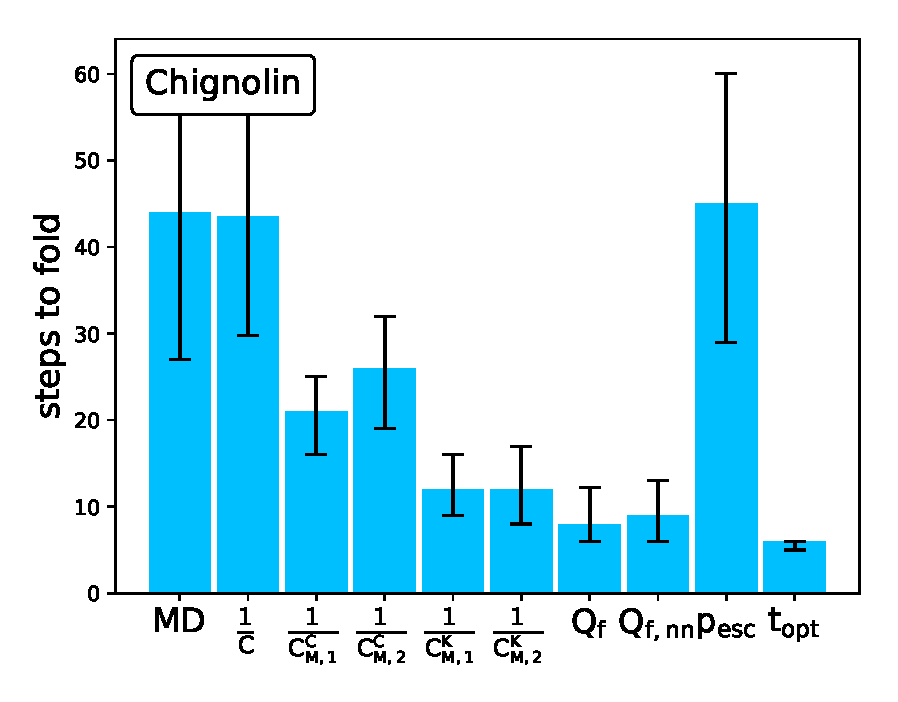
\includegraphics[width=0.9\textwidth]{figures/CLN025_7_steps10000_nparallel100_fold.eps} 
  \end{subfigure}
  \begin{subfigure}[t]{0.5\textwidth}
    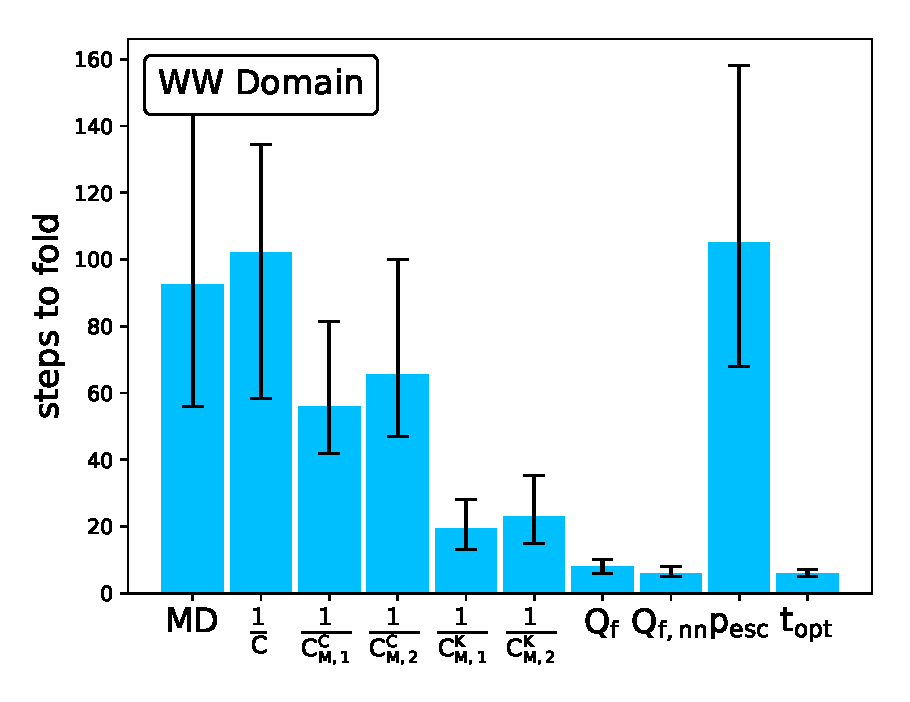
\includegraphics[width=0.9\textwidth]{figures/GTT_7_steps10000_nparallel100_fold.eps}  
  \end{subfigure}
  \begin{subfigure}[t]{0.5\textwidth}
    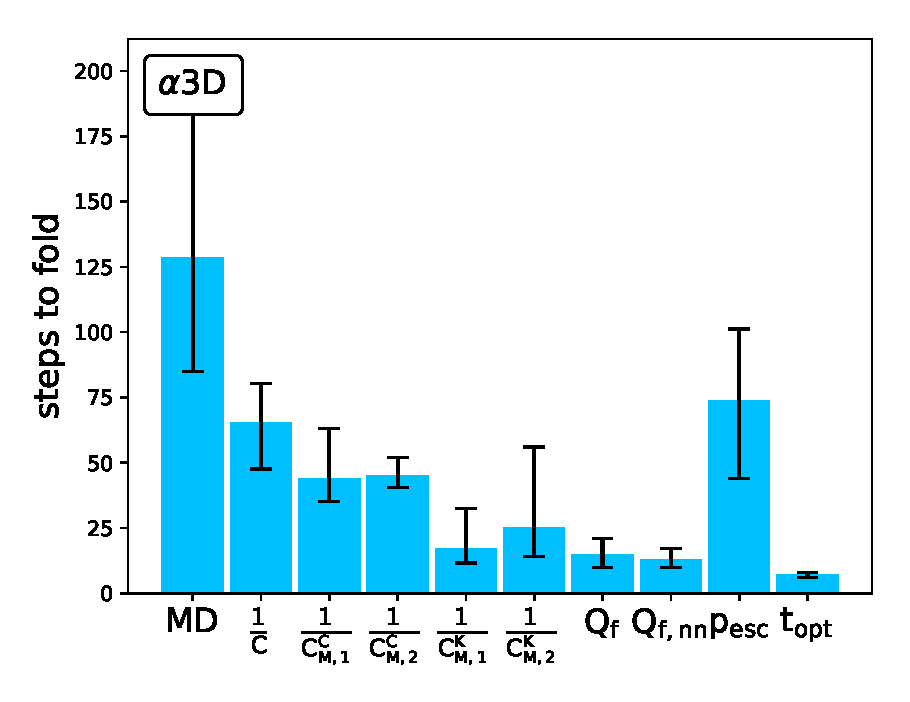
\includegraphics[width=0.9\textwidth]{figures/A3D_7_steps10000_nparallel100_fold.eps}   
  \end{subfigure}
  \caption{Time to fold for the different sampling strategies for proteins Chignolin, WW Domain and $\alpha$3D.}
  \label{fig:Time_fold}
\end{figure}


The time to fold the protein is the most common objective of adaptive sampling. Figure~\ref{fig:Time_fold} shows the performance of different adaptive sampling strategies with Markov Chain trajectories.
Each sampling strategy should be compared with plain MD, which is the reference sampling strategy.
The simple $cmicro$/$1/C$ strategy shows no speedup for Chignolin, WW Domain, and only a small 2x speedup for $\alpha$3D. This shows that the $cmicro$ strategy is not optimal for folding proteins. The reason for the low efficiency lies in the oversampling of states which are not on the folding path but have a low stationary probability and high restart probability.

The $cmacro$ strategies show a significant speedup compared to plain MD for all the proteins, but the 4 variants of the $cmacro$ strategies show significant performance differences.
Between the 4 variants of the $cmacro$ strategies, it seems the correction of the MSM due to non-equilibrium  $1/C_{K, 1}$ improves the results most. While the approximation of the Koopman method with the Markov Chain trajectories is only an upper limit for the performance improvement, the improvement is 2-3x. The improved performance of the corrected MSMs is caused by the improved estimation of the collective motions of the proteins. The estimated macrostates are kinetically more accurate. The 2 variants in setting the number of macrostates don't show a substantial performance effect. The constant number
of macrostates $1/C_{M, 1}$ is slightly faster. The underperformance of the kinetically set number of macrostates could be caused by the challenge of determining the timescales for partially sampled energy landscapes accurately

The two adaptive sampling strategies with \emph{a priori} information $Q_{f}$ and $Q_{f,nn}$ show significant improvement over $1/C_{K, 1}$, which is the best strategy without \emph{a priori} information. If the \emph{a priori} information is accurate, then this can speedup the folding of the protein significantly. Depending on the protein the improvement with the \emph{a priori} information can be less than 50
\% or a factor 2-3x. The effectivity of including the dimension of \emph{a priori} information to prevent misfolded states in  $Q_{f,nn}$ varies on the protein, but no significant performance penalties are observed.

The two benchmark strategies $p_{esc}$ and $t_{opt}$ show very different performance. The strategy optimized to fold proteins $t_{opt}$  shows the upper limit for protein folding speedup with adaptive sampling. This benchmark shows a 2x or more improvement compared to strategies with no \emph{a priori} information, allowing a gap for the improvement of adaptive sampling strategies. Previously the upper limit for performance of protein folding with adaptive sampling was unknown. The $t_{opt}$ strategy is in some proteins close to the performance of $Q_{f,nn}$, the best strategy with \emph{a priori} information. The similar performance can be caused due to the simple protein folding pathway. For other proteins, the $t_{opt}$ strategy is significantly faster than $Q_{f,nn}$, showing that adaptive sampling strategies with \emph{a priori} information have opportunities to improve. The strategy optimized to explore all states indiscriminately $p_{esc}$ isn't effective in folding proteins. The performance of the adaptive sampling strategies is consistent between different proteins, allowing to conclude that adaptive sampling is effective for different topologies, both $\alpha$-helices and $\beta$ sheets.

\subsection{\label{sec:time-explore}Time to explore 95\% of states}

\begin{figure}[H]
  %%\centering
  \begin{subfigure}[t]{0.5\textwidth}
    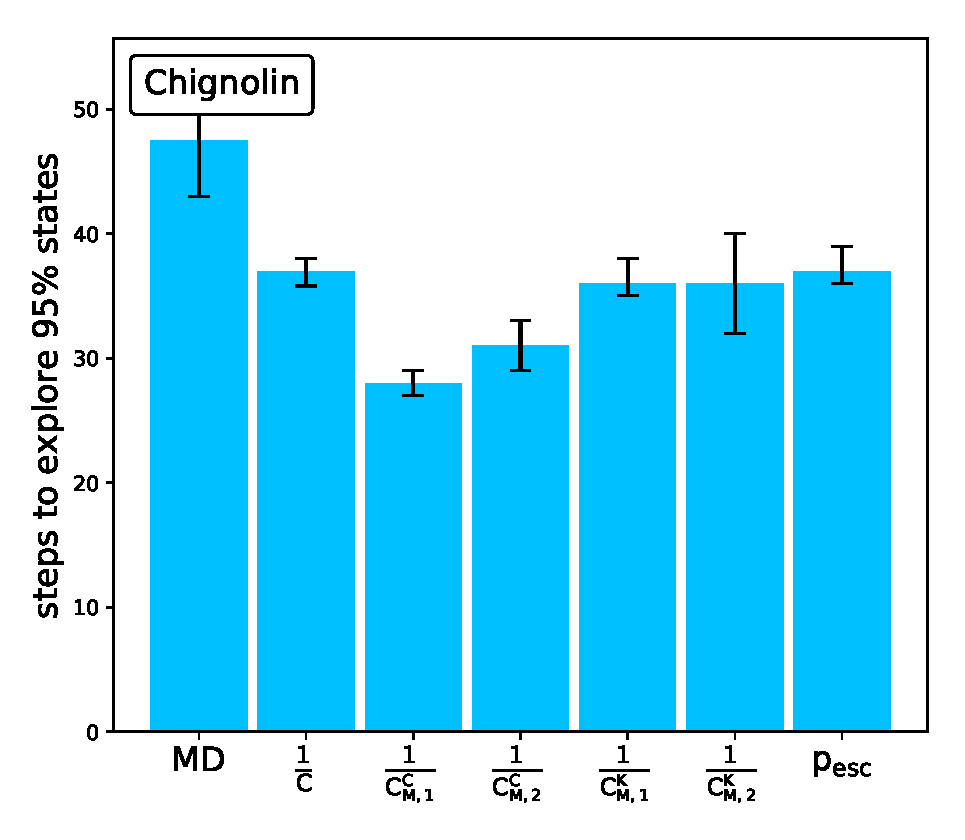
\includegraphics[width=0.9\textwidth]{figures/CLN025_7_steps10000_nparallel100_explore.eps}
  \end{subfigure}
  \begin{subfigure}[t]{0.5\textwidth}
    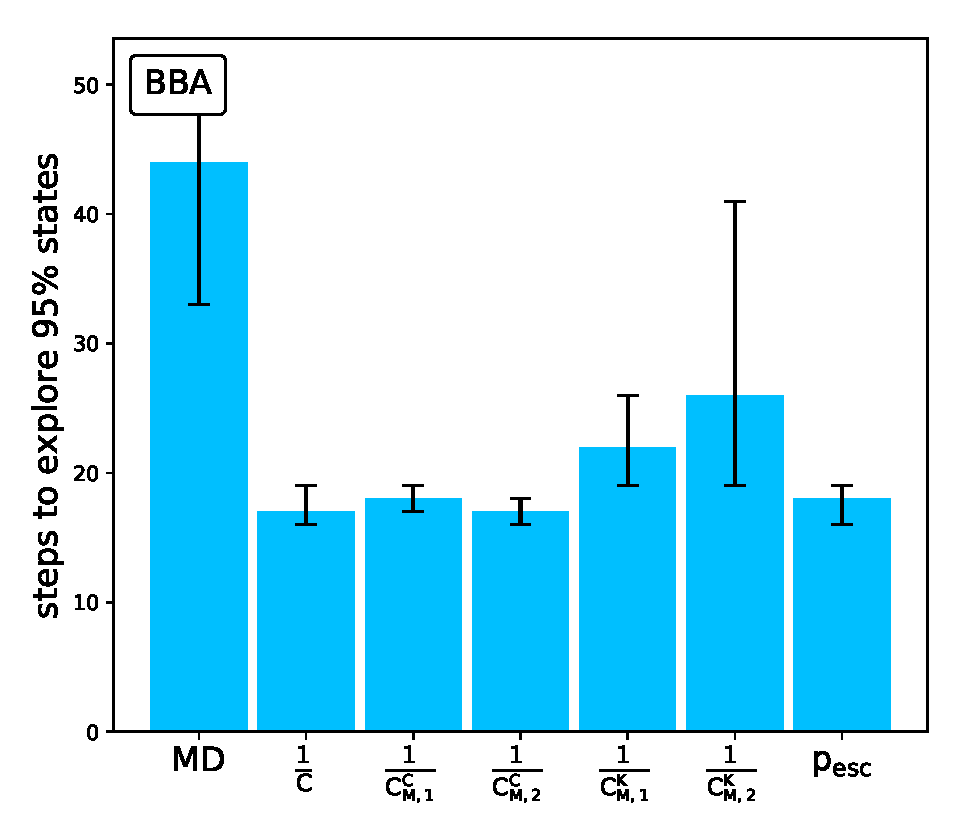
\includegraphics[width=0.9\textwidth]{figures/1FME_7_steps10000_nparallel100_explore.eps}   
  \end{subfigure}
  \begin{subfigure}[t]{0.5\textwidth}
    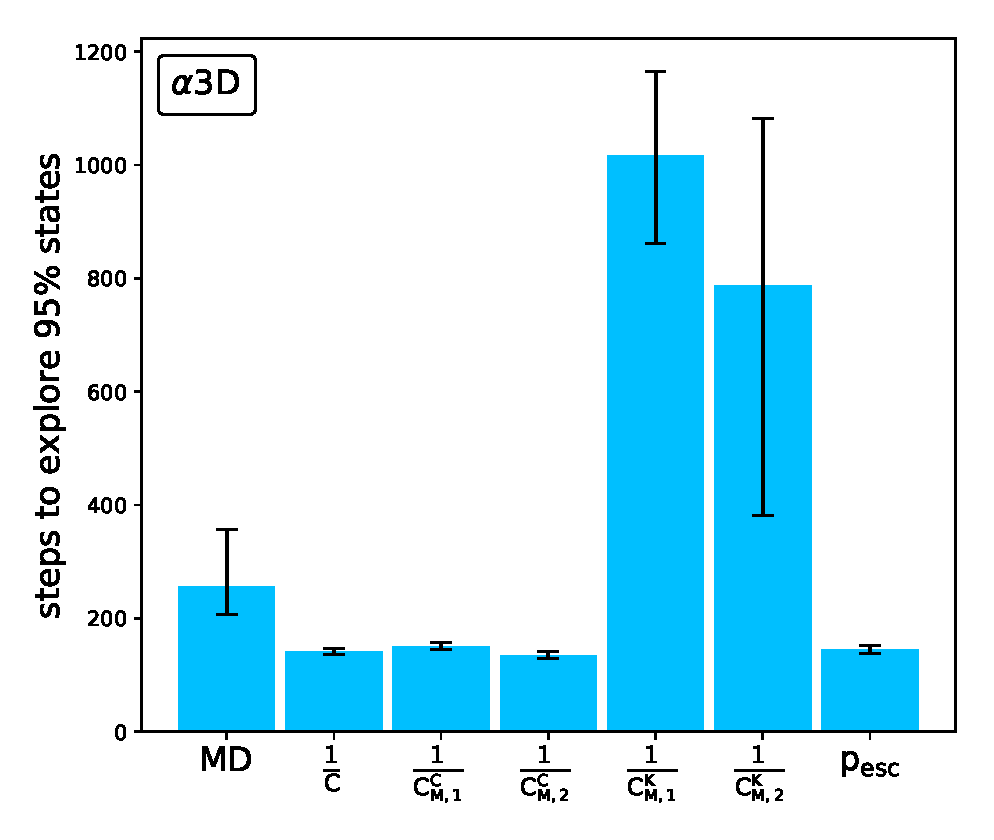
\includegraphics[width=0.9\textwidth]{figures/A3D_7_steps10000_nparallel100_explore.eps}   
  \end{subfigure}
  \caption{Time to the exploration of 95\% of the states for the different sampling strategies for proteins Chignolin, BBA and $\alpha$3D.}
  \label{fig:Time_explore}
\end{figure}

The time to explore the whole energy landscape is an alternative metric to evaluate the effectiveness of adaptive sampling. Figure~\ref{fig:Time_explore} shows the average time needed to explore 95\% of the microstates for different adaptive sampling strategies with Markov Chain trajectories.
The results show that the adaptive sampling strategies show a different performance for this metric. Comparing to the protein folding metric, the $cmicro$ strategy performs better for the exploration metric, and the $cmacro$  strategy performs relatively worse for the exploration metric. Despite the worse performance of $cmacro$, for some proteins like Chignolin, it's the fastest strategy. 


For some proteins such as Chignolin, the $p_{esc}$ strategy is slower than the $(1/C_M^C)$ strategy. This is caused by the rare transition barrier in the folding landscape. The $p_{esc}$ is a greedy algorithm and doesn't take the rare transition barrier into account. The $t_{opt}$ strategy was not shown in Fig.~\ref{fig:Time_explore}, since this strategy never explores the 95\% of the states. This is expected since this strategy is optimized for a different objective.
Surprisingly, the strategies $cmacro$ strategies with regular MSM $(1/C_M^C)$ outperform
the strategies with corrected MSM $(1/C_M^K)$. This unexpected result is probably caused by the correction, which biases the sampling towards slow processes and away from general exploration.

It's unclear which variant of the $cmacro$ strategy for the number of macrostates performs better due to the variance of performance between the proteins. For the metric of exploration, the strategies $cmicro$ or  $(1/C_M^C)$ are preferable. 

\subsection{\label{sec:scaling}Scaling}

\begin{figure}[H]
  \begin{subfigure}[t]{0.5\textwidth}
    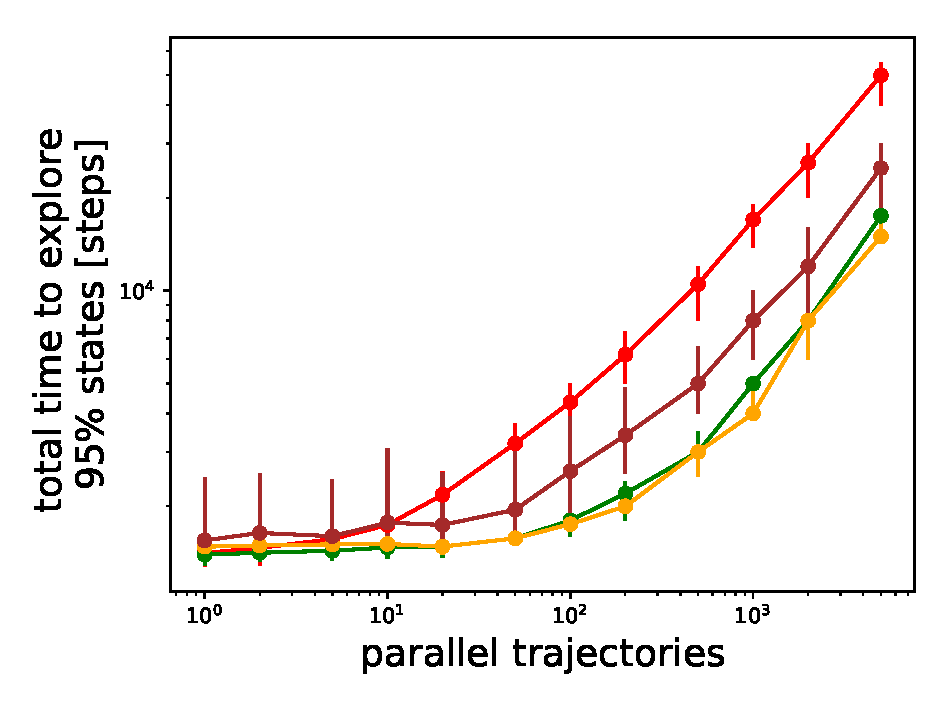
\includegraphics[width=0.9\textwidth]{figures/1FME_6_steps10000_scaling_explore_total.eps}   
  \end{subfigure}
  \begin{subfigure}[t]{0.5\textwidth}
    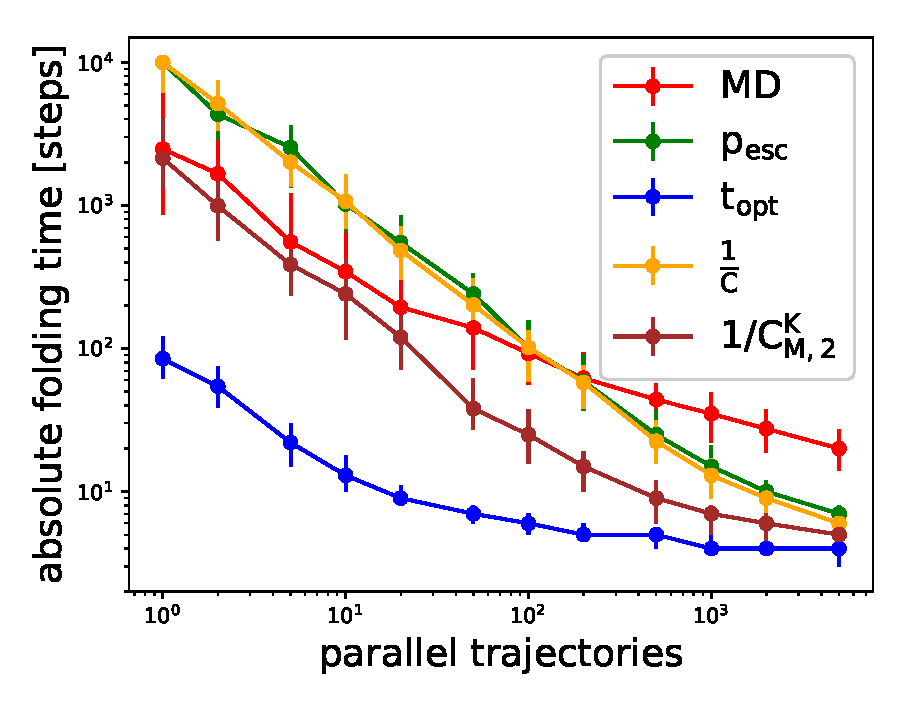
\includegraphics[width=0.9\textwidth]{figures/GTT_6_steps10000_scaling_fold0.eps}    
  \end{subfigure}
  \begin{subfigure}[t]{0.5\textwidth}
    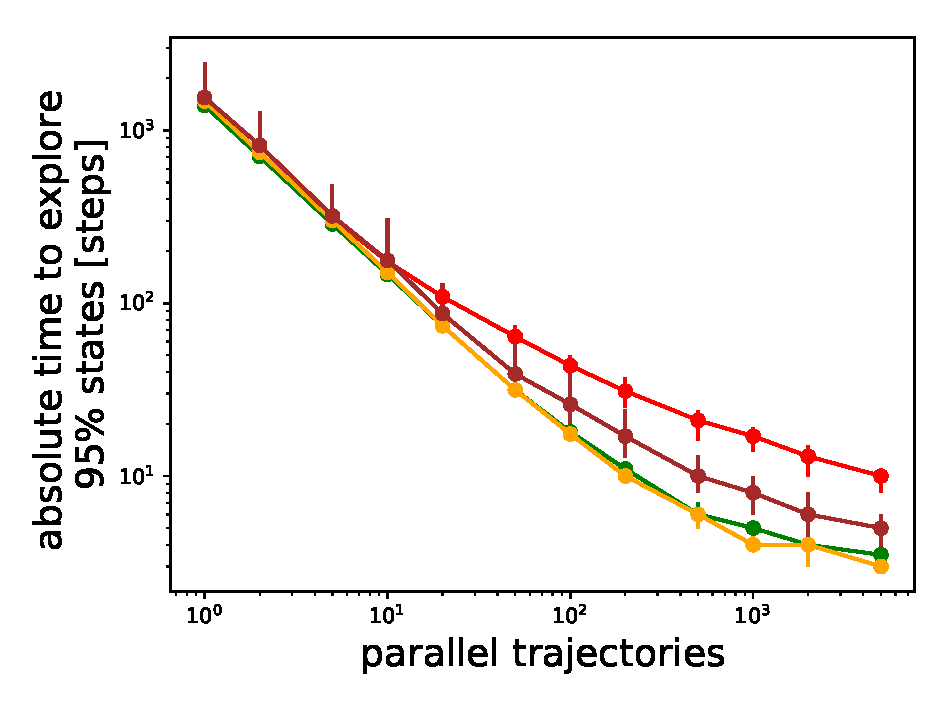
\includegraphics[width=0.9\textwidth]{figures/1FME_6_steps10000_scaling_explore.eps}   
  \end{subfigure}

  \caption{Top] Scaling of the
  absolute (left) or cumulative (right) number of steps required to explore
  95\% of all microstates. Strategies plain $MD$, $p_{esc}$, $1/C$ and $1/C_{M,2}^K$ for the protein BBA. 
  Bottom] Scaling of the absolute folding time for sampling strategies; plain
  $MD$, $p_{esc}$, $t_{opt}$, $1/C$ and $1/C_{M,2}^K$ for WW Domain.
  }
  \label{fig:scaling}
\end{figure}

The scalability of adaptive sampling is essential for both application and understanding of adaptive sampling.  Adaptive sampling is usually deployed on High-Performance Computers, which have a high parallelization available. Parallelization allows us to shorten the time to solution by dividing the work among different GPUs, but only as long adaptive sampling scales well.
The metric absolute time represents the time to solution, but is hardware and software independent and measures the length of consecutive MD simulations. The cumulative/total time represents the computational resources necessary and is hardware and software independent as well and measures the sum of all lengths of MD simulations.
Figure \ref{fig:scaling} shows how the time to folding and time to exploration depends on the parallelization. The absolute time decreases rapidly up to parallelization of 100-1000. Any higher parallelization will not decrease the time to solution. This scaling limit depends on the protein; for larger proteins, it's slightly higher. All adaptive sampling strategies scale similarly, but plain MD scales worse. This worse scaling of plain MD is explained by the lack of communication between the individual MD trajectories for plain MD. In contrast, adaptive sampling shares information between the different replicas, which allows adaptive sampling to scale better. The total time to explore shows that the computational resources necessary to sample a protein increase rapidly above the scaling limit of 100-1000. This increase of total time indicates a lower efficiency for utilization of the GPUs but could be traded off to reduce the time to solution. For plain MD, the computational resources necessary increase above 10 replicas or GPUs.



\subsection{\label{sec:compare}Speedup for different proteins}


\begin{figure}[H]
  \begin{subfigure}[t]{0.5\textwidth}
    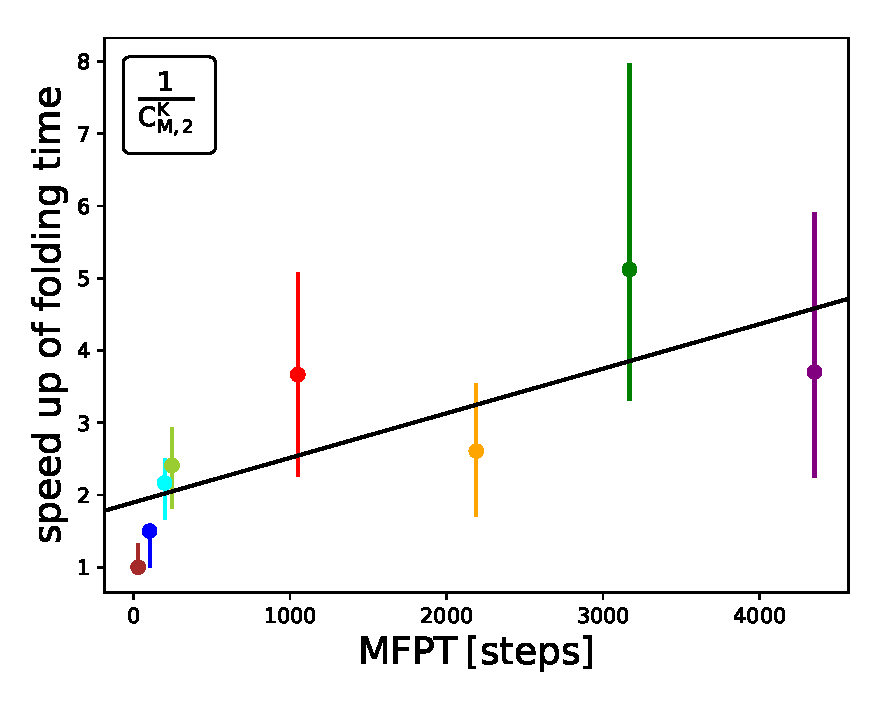
\includegraphics[width=0.9\textwidth]{figures/compare_MD_speed_up_cmacro_kin_cont_50_6_steps10000_52.eps}
  \end{subfigure}
  \begin{subfigure}[t]{0.5\textwidth}
    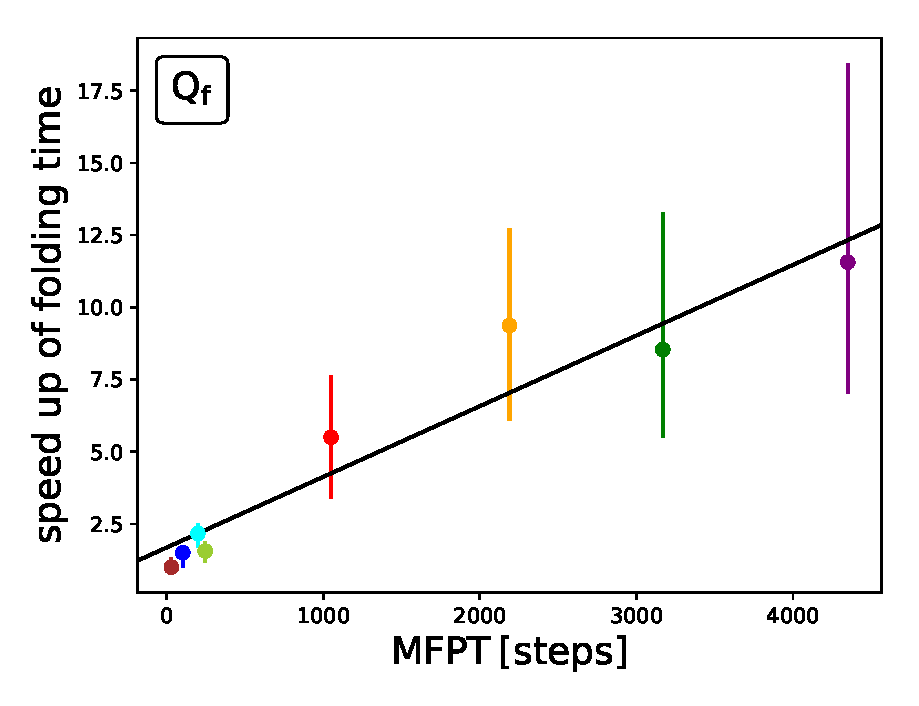
\includegraphics[width=0.9\textwidth]{figures/compare_MD_speed_up_qcore_only_6_steps10000_52.eps}   
  \end{subfigure}
    \begin{subfigure}[t]{0.5\textwidth}
    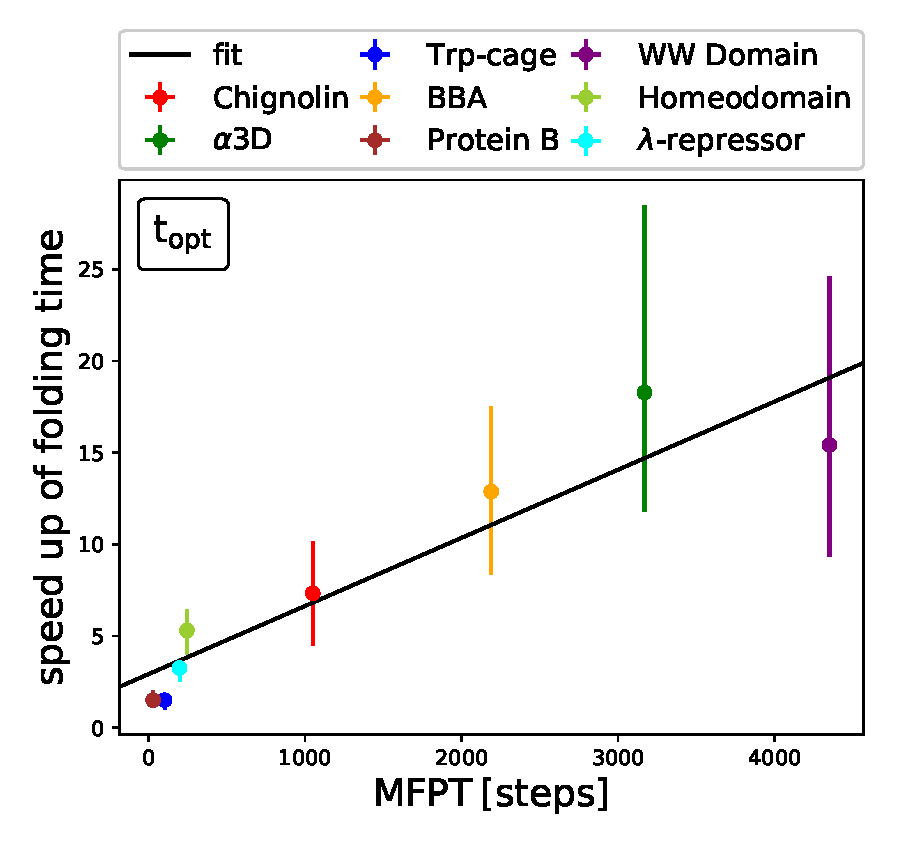
\includegraphics[width=0.9\textwidth]{figures/compare_MD_speed_up_t_opt_6_steps10000_52_0.eps}
  \end{subfigure}
  \caption{Correlation between the speedup of the folding time vs. mean first passage time for the 8 proteins and adaptive sampling strategies $1/C_{M,2}^K$, $Q_f$ and $t_{opt}$.}
  \label{fig:compare-MD-speed-cmacro}
\end{figure}

The previous figures showed a significant variance in performance between individual proteins. Plotting the speedup of folding time relative to plain MD in Figure~\ref{fig:Time_fold} allows understanding how protein size and folding time affect the adaptive sampling speedup. Despite the limited number of proteins investigated due to limited reference data, a relationship for adaptive sampling speedup is visible. The strategies shown, $1/C_{M,2}^K$, $Q_f$ and $t_{opt}$, increase the speedup with folding time for the protein. This dependency is roughly linear, with Pearson correlation coefficients is 0.82 for $1/C_{M,2}^K$, 0.95 for $Q_f$ and 0.93 for $t_{opt}$. The optimal strategy $t_{opt}$ and strategy with \emph{a priori} information have a higher correlation coefficient. The upper limit strategy for folding $t_{opt}$ reaches a speedup about 5 times of $1/C_{M,2}^K$ and about 50\% higher than $Q_f$. This shows an opportunity for improved adaptive sampling strategies. All the proteins are relatively small due to limited reference data, but the increasing speedup for longer folding and larger protein allows to predict that larger proteins can reach speedups above 10x with $1/C_{M,2}^K$. The maximal possible speedup with adaptive sampling is not known. 

\section{\label{sec:conclusion}Discussion}


This systematic analysis of adaptive sampling strategies allows comparing different strategies with an improved statistical sampling.
The effectivity of correcting the MSM for non-equilibrium sampling was demonstrated by the performance of $1/C_{M,2}^K$ for folding proteins. This result is limited by the approximation, which was used to estimate the performance of correcting the MSM with the Koopman method. For folding a protein with the $1/C_{M,2}^K$ strategy is preferable, reaching a speedup of up to 5x for the investigated small proteins. The most efficient adaptive sampling strategy is based on the iterative identification of kinetically disconnected macrostates with corrections for non-equilibrium effects.

Another result is that a different goal of the sampling, such as exploring all the states, dramatically affects the speedup with adaptive sampling strategies. For exploration $cmicro$ or  $(1/C_M^C)$ strategies are preferable. 
An unexplored consideration is the utilization of multiple strategies. At the beginning of adaptive sampling, the folding of the protein could be prioritized; later the exploration or increasing the accuracy of the kinetic results could be prioritized.

The increased effectivity of adaptive sampling strategies with \emph{a priori} knowledge about the biomolecules has been confirmed. In some cases, the speedup reaches the upper limit determined by the $t_{opt}$ strategy. These strategies can only be used when the \emph{a priori} information is accurate. Inaccurate or intuitive reaction coordinates can lead to a slower sampling of the biomolecule.

The newly developed upper limit strategy for folding time $t_{opt}$ shows the maximal speedup with adaptive sampling, which is around 15x for the investigated small proteins. Increased speedups are predicted for larger and slower folding proteins. The second upper limit strategy for exploration $p_{esc}$ is not a good benchmark since, in some cases, the $cmacro$ strategy performed better. This is caused by the greedy algorithm nature of this upper limit strategy.

The significant performance gap between the $1/C_{M,2}^K$ strategy, and the upper limit $t_{opt}$ shows an opportunity for more effective adaptive sampling strategies.

Unexpectedly, plain MD simulations with a larger number of replicas than 100 increase the required computational resources, which shows a disadvantage of plain MD compared to adaptive sampling. Adaptive sampling scales well to 100-1000 replicas; this extends the results of \cite{bowman2010enhanced} for different proteins.  

The results in this Chapter are limited by the approximation of molecular dynamics trajectories by Markov chain trajectories. This approximation allowed us to increase the sample size of adaptive sampling by several orders of magnitude but also introduces the inaccuracies of the generated MSM model. These inaccuracies of the MSM models were limited by the careful generation of the MSM models. Additionally, the effect of the Koopman method could only be approximated.

This result is encouraging for using adaptive sampling for a higher number of replicas and larger, more complex proteins. Currently, adaptive sampling is limited by the significant computational resources to fold larger proteins. The cautious extrapolation of the adaptive sampling speedup for protein folding allows predicting speedup of excess of 10-times for larger proteins.











